% !TEX program = pdflatex
% Overleaf: upload presentation-overleaf folder (or presentation-overleaf.zip)
% 22 slides | Abiy Alemu & Natnael Abayneh | AAU M.Sc. AI

\documentclass[aspectratio=169,11pt]{beamer}

\usetheme{Madrid}
\usecolortheme{default}
\usefonttheme{professionalfonts}
\useinnertheme{circles}

\definecolor{AAUBlue}{HTML}{003366}
\definecolor{AAUGold}{HTML}{C4A035}
\definecolor{AccentTeal}{HTML}{00897B}
\definecolor{SoftBg}{HTML}{F4F7FA}
\definecolor{TextGray}{HTML}{37474F}

\setbeamercolor{structure}{fg=AAUBlue}
\setbeamercolor{palette primary}{bg=AAUBlue,fg=white}
\setbeamercolor{palette secondary}{bg=AccentTeal,fg=white}
\setbeamercolor{palette tertiary}{bg=AAUGold,fg=white}
\setbeamercolor{title}{fg=AAUBlue}
\setbeamercolor{frametitle}{bg=AAUBlue,fg=white}
\setbeamercolor{block title}{bg=AccentTeal,fg=white}
\setbeamercolor{block body}{bg=SoftBg,fg=TextGray}
\setbeamercolor{alerted text}{fg=AAUGold}

\setbeamertemplate{navigation symbols}{}
\setbeamertemplate{footline}{%
  \leavevmode%
  \hbox{%
    \begin{beamercolorbox}[wd=.45\paperwidth,ht=2.6ex,dp=1.2ex,leftskip=1em]{author in head/foot}%
      \usebeamerfont{author in head/foot}\insertshortauthor
    \end{beamercolorbox}%
    \begin{beamercolorbox}[wd=.35\paperwidth,ht=2.6ex,dp=1.2ex,center]{title in head/foot}%
      \usebeamerfont{title in head/foot}\insertshorttitle
    \end{beamercolorbox}%
    \begin{beamercolorbox}[wd=.2\paperwidth,ht=2.6ex,dp=1.2ex,rightskip=1em]{date in head/foot}%
      \usebeamerfont{date in head/foot}\insertframenumber{} / 22
    \end{beamercolorbox}%
  }%
  \vskip0pt%
}

\usepackage[T1]{fontenc}
\usepackage{lmodern}
\usepackage{amsmath,amssymb}
\usepackage{booktabs}
\usepackage{graphicx}
\usepackage[table]{xcolor}
\usepackage{tikz}
\usepackage{tcolorbox}
\usepackage{hyperref}
\usetikzlibrary{arrows.meta, positioning}

\tcbset{
  colback=SoftBg, colframe=AccentTeal, fonttitle=\bfseries,
  boxrule=0.6pt, arc=2pt, left=4pt, right=4pt, top=3pt, bottom=3pt
}

% Full-slide figure helper
\newcommand{\bigfig}[2][]{%
  \begin{center}
    \includegraphics[#1,width=0.92\textwidth,height=0.76\textheight,keepaspectratio]{#2}
  \end{center}
}

\title[Heart Disease BN]{Medical Diagnosis System Using\\Bayesian Networks for Heart Disease Prediction}
\subtitle{Probabilistic Graphical Models (PGM) Course Project}
\author[Abiy \& Natnael]{Abiy Alemu \and Natnael Abayneh}
\institute[AAU]{Addis Ababa University\\M.Sc.\ in Artificial Intelligence}
\date{June 2026}

\begin{document}

% --- 1. Title ----------------------------------------------------------------
\begin{frame}[plain]
  \titlepage
  \vspace{-0.6cm}
  \begin{center}\small\textcolor{TextGray}{Educational research demo --- not for clinical use}\end{center}
\end{frame}

% --- 2. Motivation -----------------------------------------------------------
\begin{frame}{Motivation \& Problem Statement}
  \begin{columns}[T]
    \column{0.58\textwidth}
    \begin{alertblock}{Core question}
      \Large
      $P(\text{Heart Disease} \mid \text{symptoms, vitals, tests})$
    \end{alertblock}
    \vspace{0.4em}
    \begin{itemize}
      \item Heart disease diagnosis relies on \textbf{multiple uncertain} clinical signals.
      \item Clinicians update belief as new evidence arrives.
      \item We need \textbf{interpretable} probabilistic reasoning --- not a black box.
    \end{itemize}
    \column{0.40\textwidth}
    \begin{block}{Why Bayesian Networks?}
      \begin{itemize}
        \item Explicit DAG \textbf{representation}
        \item Parameters \textbf{learned} from data
        \item Exact \textbf{inference} for $P(\text{disease}\mid\mathbf{e})$
        \item Handles partial / missing evidence
      \end{itemize}
    \end{block}
  \end{columns}
\end{frame}

% --- 3. Objectives -----------------------------------------------------------
\begin{frame}{Project Objectives}
  \begin{enumerate}
    \item \textbf{Represent} medical knowledge as Bayesian Network DAGs.
    \item \textbf{Learn} CPTs from the UCI Heart Disease dataset.
    \item \textbf{Infer} disease probability with Variable Elimination \& Belief Propagation.
    \item \textbf{Evaluate} accuracy, precision, recall, F1, and ROC-AUC.
    \item \textbf{Deploy} an interactive Streamlit demo on GitHub / Streamlit Cloud.
  \end{enumerate}
  \vspace{0.8em}
  \begin{center}
    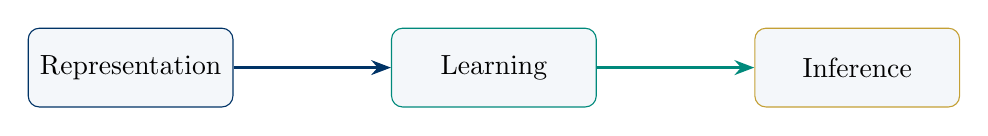
\begin{tikzpicture}[node distance=2cm, every node/.style={font=\normalsize}]
      \node[draw=AAUBlue, fill=SoftBg, rounded corners, minimum width=2.6cm, minimum height=1cm] (r) {Representation};
      \node[draw=AccentTeal, fill=SoftBg, rounded corners, minimum width=2.6cm, minimum height=1cm, right=of r] (l) {Learning};
      \node[draw=AAUGold, fill=SoftBg, rounded corners, minimum width=2.6cm, minimum height=1cm, right=of l] (i) {Inference};
      \draw[-{Stealth[length=2.5mm]}, line width=1.2pt, AAUBlue] (r) -- (l);
      \draw[-{Stealth[length=2.5mm]}, line width=1.2pt, AccentTeal] (l) -- (i);
    \end{tikzpicture}
  \end{center}
\end{frame}

% --- 4. Dataset --------------------------------------------------------------
\begin{frame}{Dataset \& Preprocessing}
  \begin{columns}[T]
    \column{0.48\textwidth}
    \textbf{UCI Heart Disease} --- four clinical sources
    \vspace{0.3em}
    \begin{table}
      \begin{tabular}{@{}lr@{}}
        \toprule
        Source & Patients \\
        \midrule
        Cleveland & 303 \\
        Hungarian & 294 \\
        Switzerland & 123 \\
        VA Long Beach & 200 \\
        \midrule
        \textbf{Total} & \textbf{920} \\
        \bottomrule
      \end{tabular}
    \end{table}
    \small 13 features + binary label \quad|\quad 55.3\% prevalence
    \column{0.50\textwidth}
    \begin{block}{Preprocessing}
      \begin{itemize}
        \item Discretise age, BP, cholesterol, heart rate, ST depression
        \item Binary clinical encoding (optimized Cleveland model)
        \item Impute missing values as \texttt{Unknown} $\rightarrow$ train mode
        \item Stratified 75/25 train--test (+ validation for threshold tuning)
      \end{itemize}
    \end{block}
  \end{columns}
\end{frame}

% --- 5. Representation overview ----------------------------------------------
\begin{frame}{PGM Pillar I --- Representation (Four BN Models)}
  \begin{table}
    \centering
    \begin{tabular}{@{}lll@{}}
      \toprule
      \textbf{Model} & \textbf{Structure source} & \textbf{Purpose} \\
      \midrule
      Manual Structure BN & 16-edge hand-built DAG & Interpretability \\
      Naive Bayes BN & All features $\rightarrow$ disease & Classic diagnosis \\
      Chow-Liu Tree BN & Mutual-information tree & Multi-source baseline \\
      Optimized Clinical BN & Cleveland + binary features & Best accuracy \\
      \bottomrule
    \end{tabular}
  \end{table}
  \vspace{0.6em}
  \begin{center}
    \textit{Each model is a directed acyclic graph (DAG) with learned conditional probability tables.}
  \end{center}
\end{frame}

% --- 6. Manual Structure & Naive Bayes (text) ------------------------------------------
\begin{frame}{Manual Structure BN \& Naive Bayes BN}
  \begin{columns}[T]
    \column{0.50\textwidth}
    \textbf{Manual Structure BN}
    \begin{itemize}
      \item DAG built \textbf{by hand} (PGM Representation pillar)
      \item Age influences Chol, Trestbps, Thalach
      \item CP, Exang, Ca, Thal $\rightarrow$ HeartDisease
      \item Illustrates fixed structure + learned CPTs on multi-source UCI data
      \item Chow-Liu tree: \textbf{76.5\%} accuracy, \textbf{96\%} recall
    \end{itemize}
    \vspace{0.5em}
    \textbf{Naive Bayes Diagnosis BN}
    \begin{itemize}
      \item $P(D \mid \mathbf{X}) \propto P(D)\prod_i P(X_i \mid D)$
      \item 13 symptom nodes as direct parents of disease
      \item Standard PGM pattern for medical diagnosis
    \end{itemize}
    \column{0.48\textwidth}
    \begin{block}{Key idea}
      Manual Structure BN = \textbf{representation-driven} DAG.

      Naive Bayes = \textbf{diagnosis-driven} structure.

      Both learn CPTs from data via MLE + Laplace smoothing.
    \end{block}
  \end{columns}
\end{frame}

% --- 7. Manual Structure & Naive DAG figures --------------------------------------
\begin{frame}{Network Structures --- Manual Structure \& Naive Bayes}
  \begin{columns}[c]
    \column{0.49\textwidth}
    \centering
    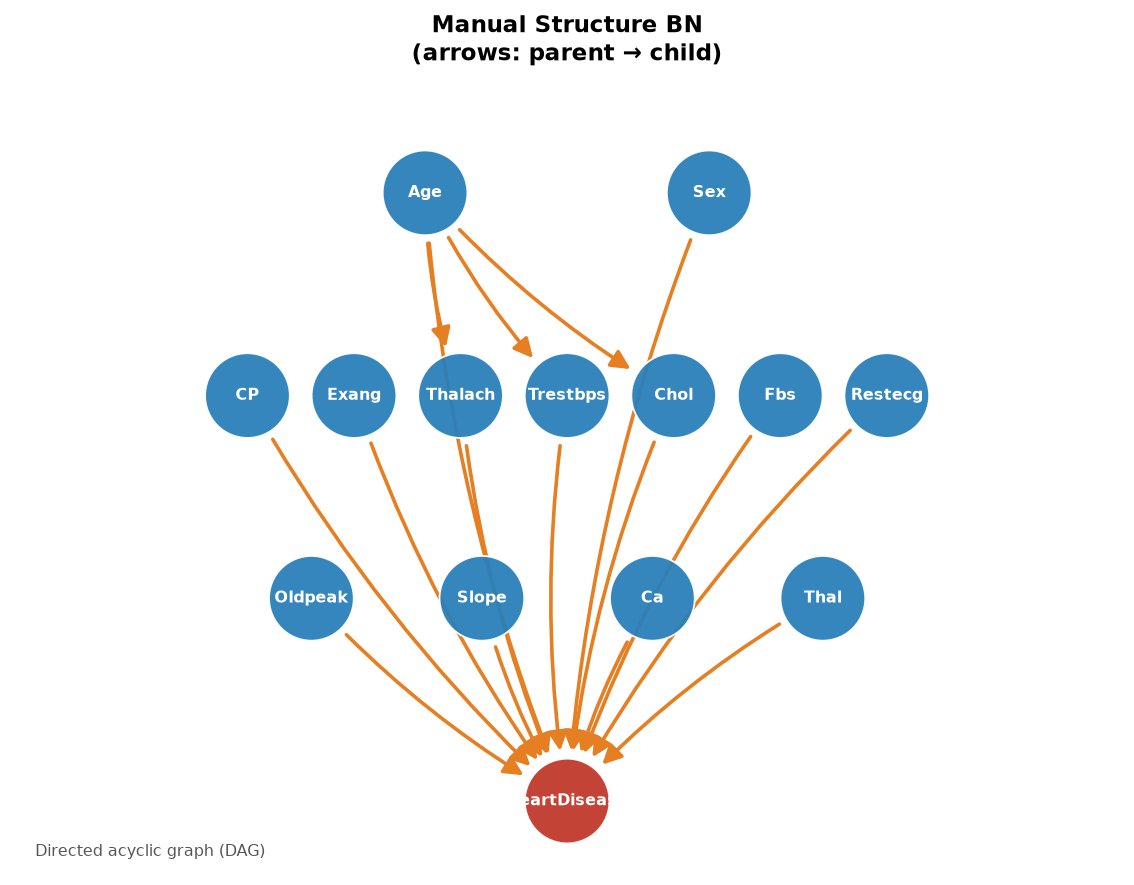
\includegraphics[width=\linewidth,height=0.72\textheight,keepaspectratio]{figures/fig0_manual_structure_dag.png}\\[0.15em]
    {\small\textbf{Manual Structure BN}}
    \column{0.49\textwidth}
    \centering
    
\includegraphics[width=\linewidth,height=0.72\textheight,keepaspectratio]{figures/fig1_naive_bayes_dag.png}\\[0.15em]
    {\small\textbf{Naive Bayes Diagnosis BN}}
  \end{columns}
\end{frame}

% --- 8. Chow-Liu & Optimized (text) ------------------------------------------
\begin{frame}{Chow-Liu Tree \& Optimized Clinical BN}
  \begin{columns}[T]
    \column{0.50\textwidth}
    \textbf{Chow-Liu Tree BN}
    \begin{itemize}
      \item Structure \textbf{learned} from data (pgmpy \texttt{TreeSearch})
      \item Maximum spanning tree weighted by mutual information
      \item Best multi-source model: \textbf{76.5\%} accuracy, \textbf{89\%} AUC
    \end{itemize}
    \vspace{0.5em}
    \textbf{Optimized Clinical BN} \textcolor{AAUGold}{$\star$ primary}
    \begin{itemize}
      \item Cleveland subset (303 patients, 10 binary features)
      \item Chow-Liu tree + $\alpha=0.05$ Laplace smoothing
      \item Balanced threshold $\tau=0.425$ on train+validation
      \item \textbf{All metrics $\geq$ 85\%} on held-out test set
    \end{itemize}
    \column{0.48\textwidth}
    \begin{block}{Optimized features}
      \small
      CP, Ca, Thal, Exang, STHigh, Sex, HRLow, AgeOld, CholHigh, BPHigh
    \end{block}
    \vspace{0.3em}
    \begin{exampleblock}{Why Cleveland-only?}
      \small Multi-source UCI data is heterogeneous; focused subset yields cleaner structure learning and higher accuracy.
    \end{exampleblock}
  \end{columns}
\end{frame}

% --- 9. NEW: Optimized DAG full slide ----------------------------------------
\begin{frame}{Optimized Clinical BN --- Learned Structure}
  \bigfig{figures/fig1c_optimized_dag.png}
  \vspace{-0.4em}
  \begin{center}
    \small Chow-Liu tree on Cleveland binary features \quad|\quad
    \textbf{Acc.\ 89.5\%} \quad \textbf{AUC 92.5\%}
  \end{center}
\end{frame}

% --- 10. Learning ------------------------------------------------------------
\begin{frame}{PGM Pillar II --- Learning}
  \begin{columns}[T]
    \column{0.48\textwidth}
    \begin{block}{Maximum Likelihood Estimation}
      \[
        \hat{\theta}_{ijk} = \frac{N_{ijk}}{N_{ij}}
      \]
      CPT entries from count frequencies in discretised training data.
    \end{block}
    \begin{block}{Laplace smoothing}
      \[
        \hat{\theta}_{ijk} = \frac{N_{ijk} + \alpha}{N_{ij} + \alpha \cdot r_i}
      \]
      Prevents zero probabilities for unseen combinations.
    \end{block}
    \column{0.48\textwidth}
    \begin{block}{Implementation}
      \begin{itemize}
        \item \textbf{pgmpy} \texttt{DiscreteBayesianNetwork}
        \item Sequential CPT fitting (avoids joblib hangs)
        \item Chow-Liu \texttt{TreeSearch} with \texttt{class\_node}=HeartDisease
        \item BIC score for structure comparison
      \end{itemize}
    \end{block}
  \end{columns}
\end{frame}

% --- 11. Inference -----------------------------------------------------------
\begin{frame}{PGM Pillar III --- Inference}
  \begin{columns}[T]
    \column{0.50\textwidth}
    \begin{block}{Variable Elimination (VE)}
      \begin{itemize}
        \item \textbf{Exact} inference on discrete BNs
        \item Sum-product elimination of non-query nodes
        \item $\sim$1\,ms per query on our models
      \end{itemize}
    \end{block}
    \begin{block}{Belief Propagation (BP)}
      \begin{itemize}
        \item Message passing; compared with VE in demo
        \item Posteriors should agree on the same DAG
      \end{itemize}
    \end{block}
    \column{0.46\textwidth}
    \begin{tcolorbox}[title=Decision rule]
      \[
        \hat{y} = \mathbb{1}\big[P(\text{Yes}\mid\mathbf{e}) \geq \tau\big]
      \]
      Threshold $\tau$ tuned for balanced accuracy, precision, recall, and F1.
    \end{tcolorbox}
    \vspace{0.3em}
    \begin{alertblock}{Explainability}
      \small Sensitivity analysis, inference traces, VE vs BP comparison in Streamlit.
    \end{alertblock}
  \end{columns}
\end{frame}

% --- 11b. EDA ----------------------------------------------------------------
\begin{frame}{Exploratory Data Analysis (Cleveland)}
  \bigfig{figures/fig_eda_dashboard.png}
  \vspace{-0.4em}
  \begin{center}\small Age, cholesterol, chest pain, correlation matrix, and target distribution --- UCI Cleveland subset\end{center}
\end{frame}

% --- 11c. Layered DAG --------------------------------------------------------
\begin{frame}{Manual Structure BN --- Layered Clinical Structure}
  \bigfig{figures/fig0b_manual_layered_dag.png}
  \vspace{-0.4em}
  \begin{center}\small Demographics $\rightarrow$ risk factors $\rightarrow$ clinical findings $\rightarrow$ HeartDisease\end{center}
\end{frame}

% --- 11d. Inference scenarios ------------------------------------------------
\begin{frame}{Probabilistic Inference Under Evidence}
  \bigfig{figures/fig_inference_scenarios.png}
  \vspace{-0.4em}
  \begin{center}\small Posterior $P(\text{Heart Disease}\mid\text{evidence})$ for prior, symptoms, and risk profiles\end{center}
\end{frame}

% --- 11e. CPT & MLE vs Bayesian --------------------------------------------
\begin{frame}{CPT Analysis \& Parameter Learning Comparison}
  \begin{columns}[c]
    \column{0.52\textwidth}
    \centering
    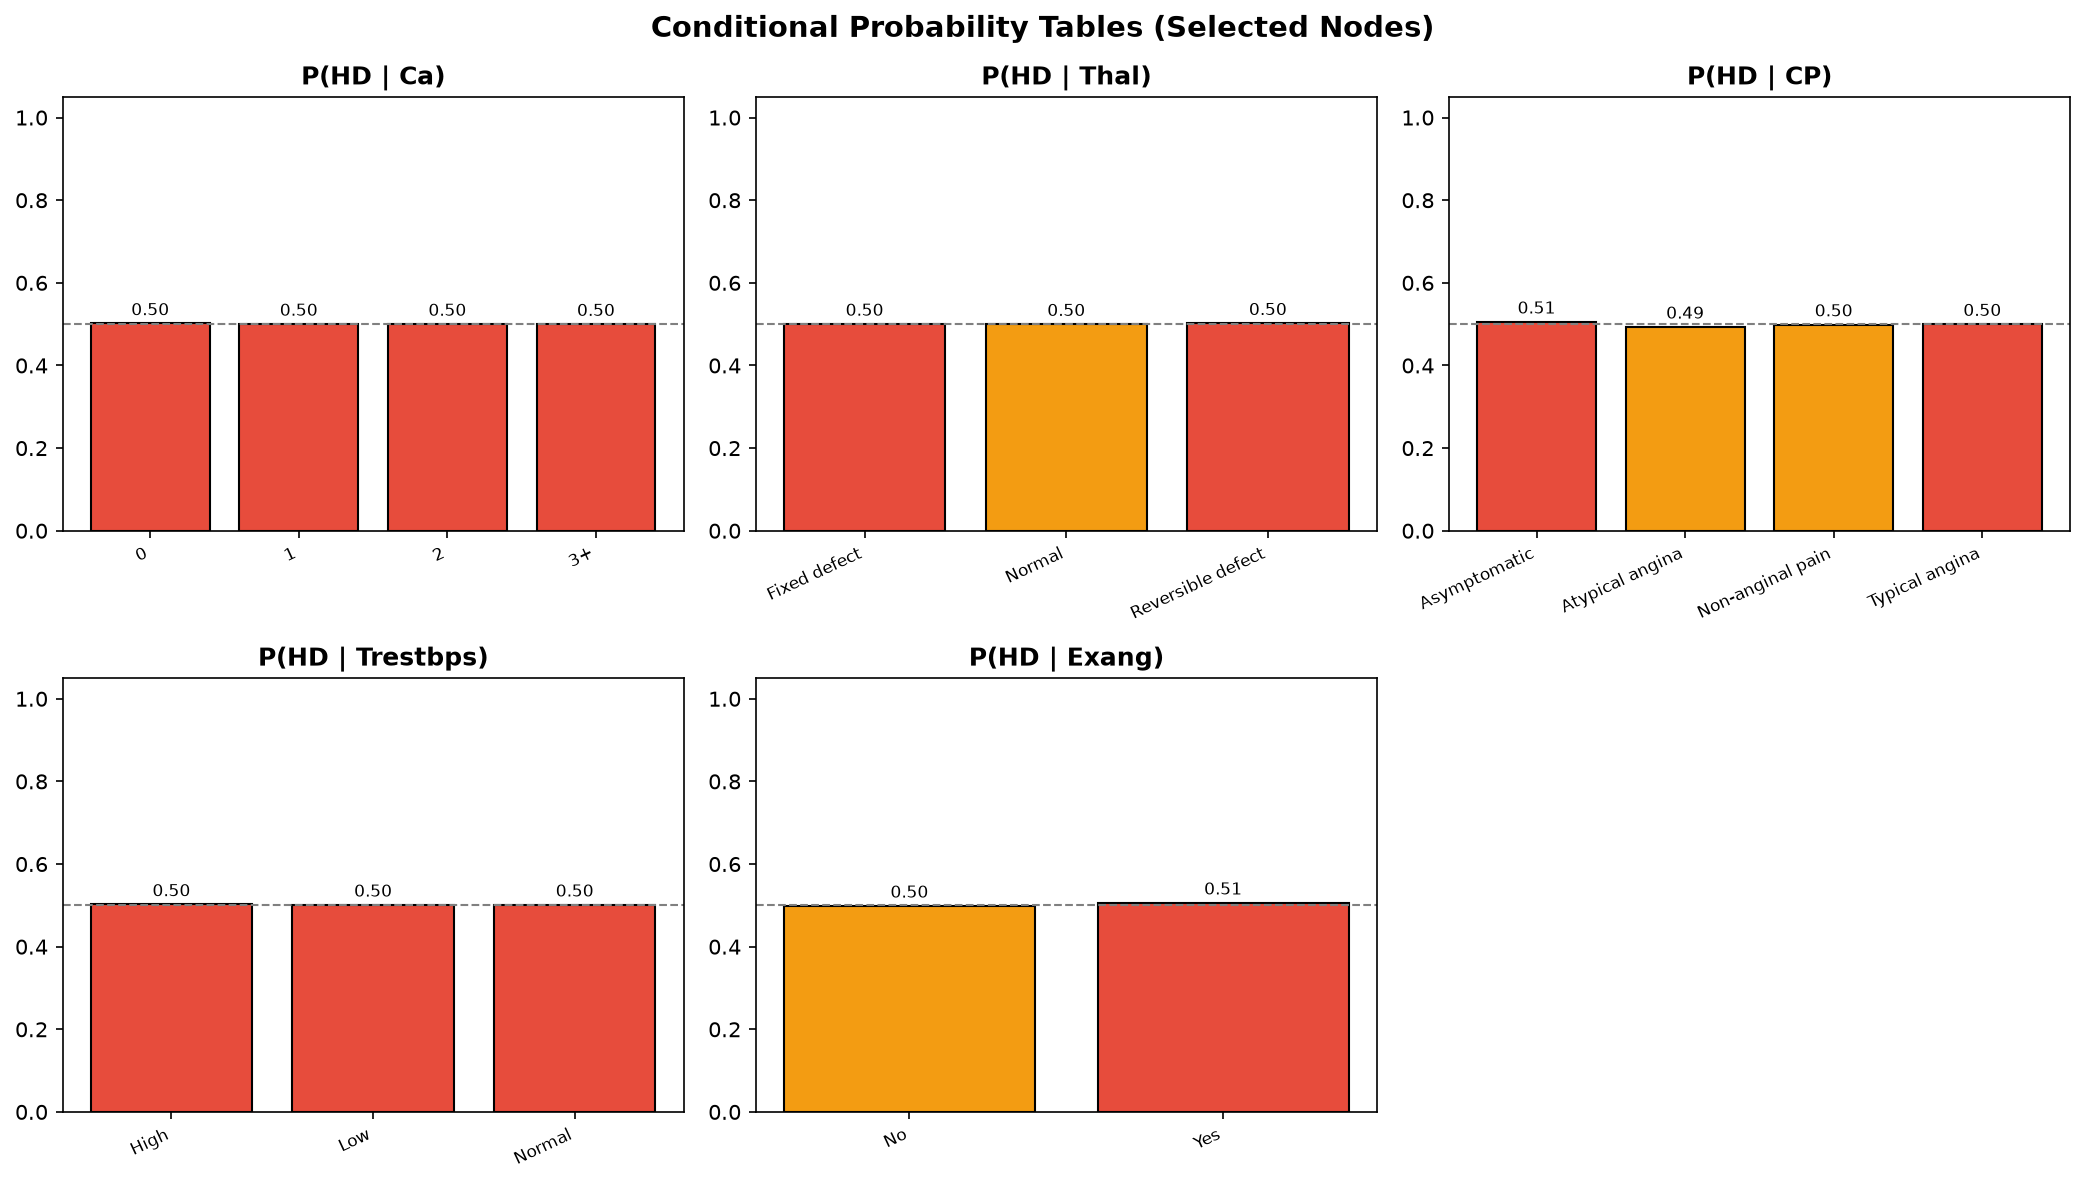
\includegraphics[width=\linewidth,height=0.68\textheight,keepaspectratio]{figures/fig_cpt_analysis.png}\\[0.15em]
    {\small\textbf{Conditional probabilities $P(\text{HD}\mid\text{feature})$}}
    \column{0.46\textwidth}
    \centering
    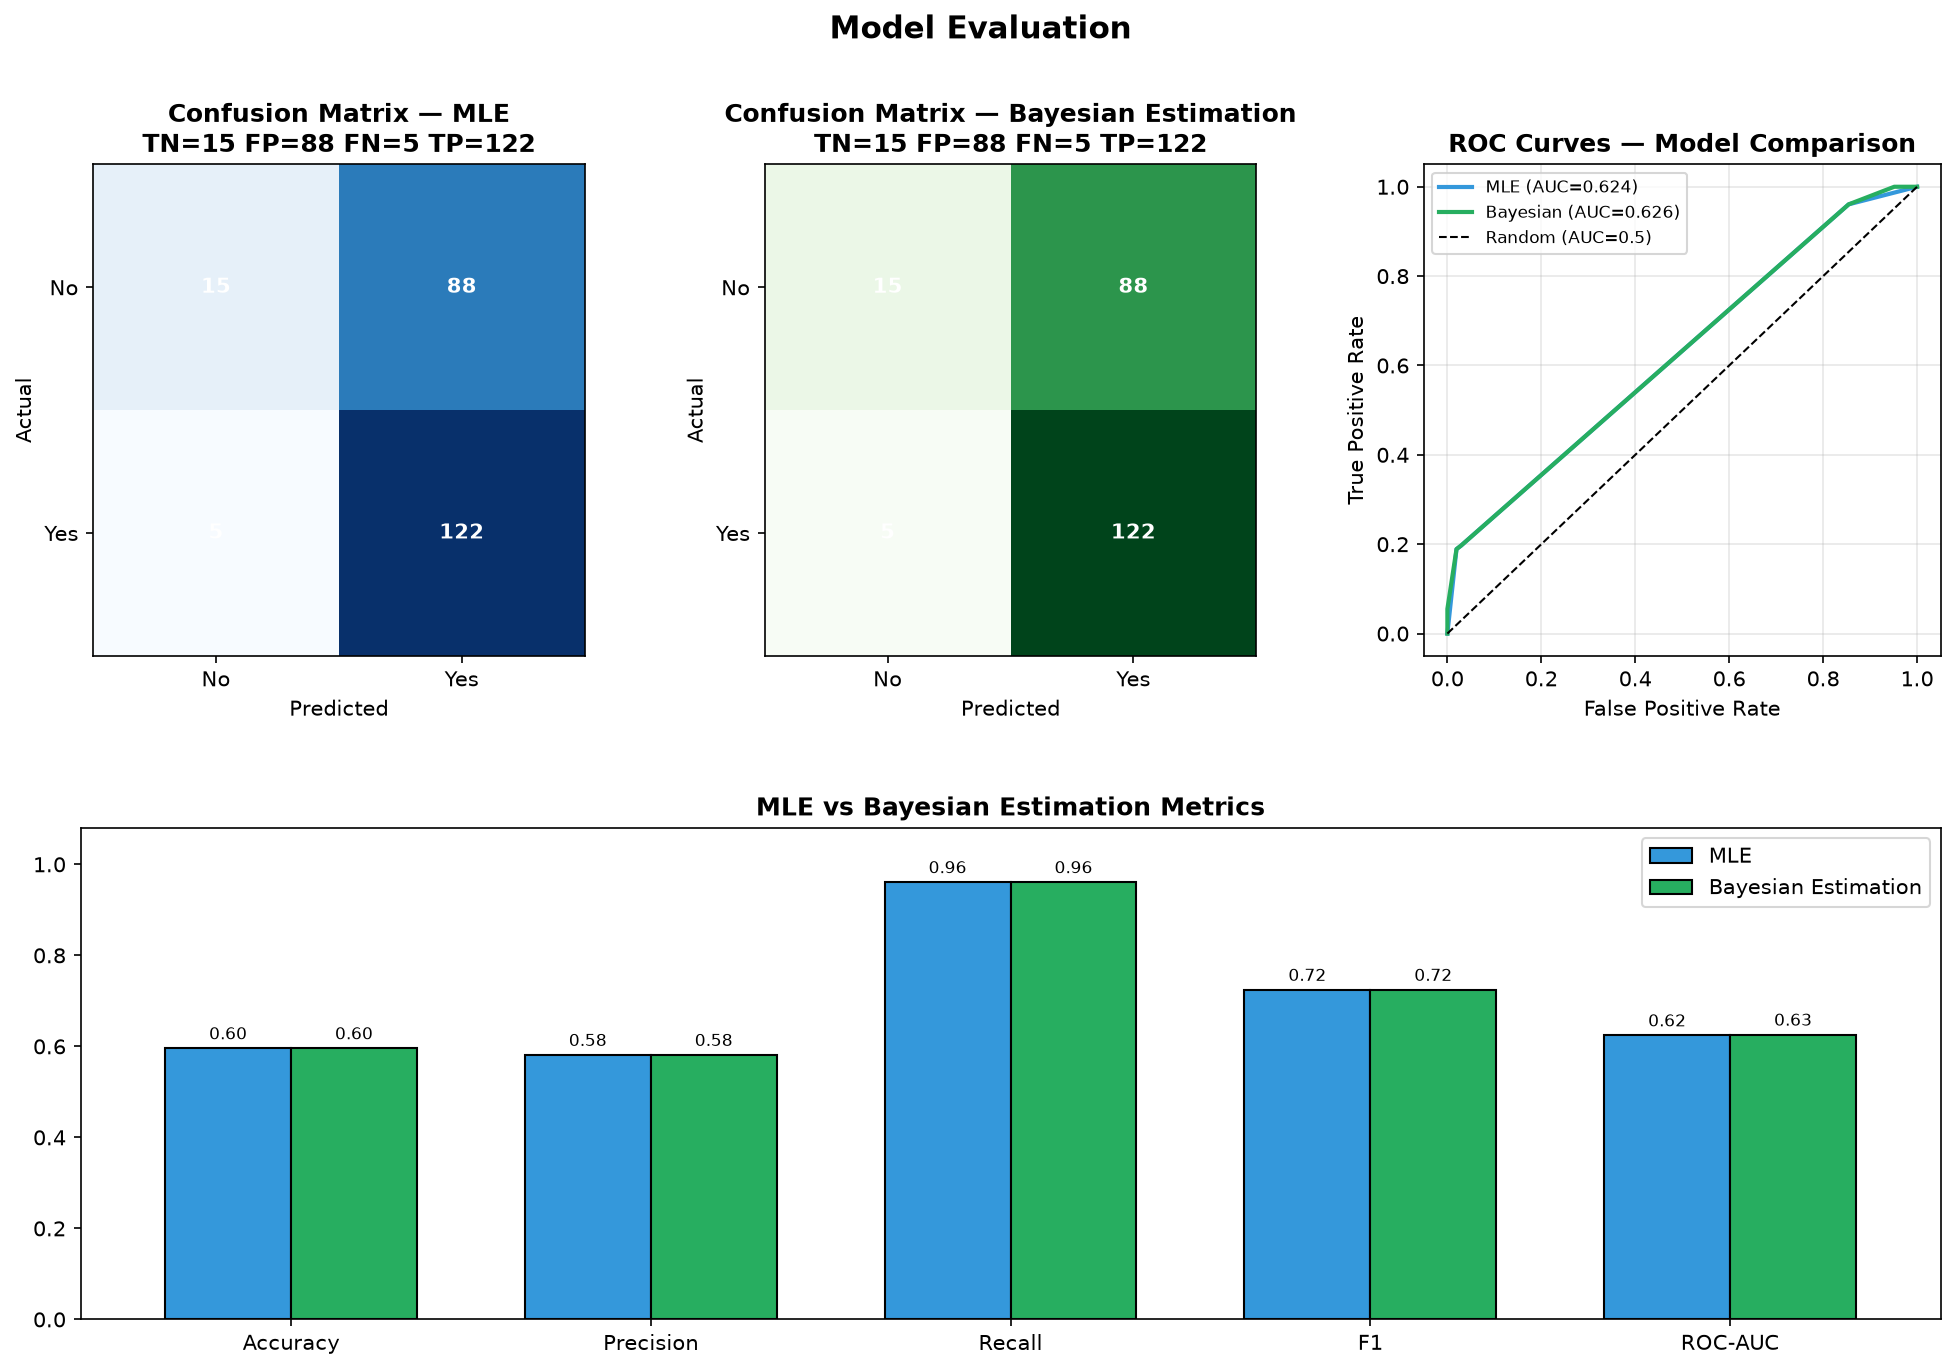
\includegraphics[width=\linewidth,height=0.68\textheight,keepaspectratio]{figures/fig_mle_vs_bayesian.png}\\[0.15em]
    {\small\textbf{MLE vs Bayesian estimation --- Manual Structure BN}}
  \end{columns}
\end{frame}

% --- 12. Pipeline ------------------------------------------------------------
\begin{frame}{End-to-End Pipeline \& Deployment}
  \begin{center}
    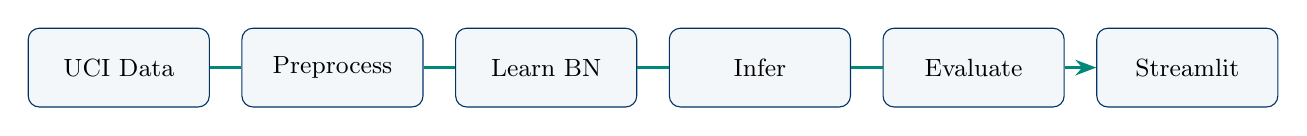
\begin{tikzpicture}[
      node distance=0.55cm and 0.4cm,
      box/.style={draw=AAUBlue, fill=SoftBg, rounded corners, minimum height=1cm, minimum width=2.3cm, font=\small, align=center}
    ]
      \node[box] (data) {UCI Data};
      \node[box, right=of data] (prep) {Preprocess};
      \node[box, right=of prep] (learn) {Learn BN};
      \node[box, right=of learn] (inf) {Infer};
      \node[box, right=of inf] (eval) {Evaluate};
      \node[box, right=of eval] (app) {Streamlit};
      \draw[-{Stealth}, line width=1pt, AccentTeal] (data) -- (prep) -- (learn) -- (inf) -- (eval) -- (app);
    \end{tikzpicture}
  \end{center}
  \vspace{0.6em}
  \begin{columns}[T]
    \column{0.50\textwidth}
    \textbf{Deliverables}
    \begin{itemize}
      \item \texttt{run.py} --- automated PGM pipeline
      \item \texttt{app/streamlit\_app.py} --- interactive demo
      \item Jupyter notebook + metrics / figures in \texttt{outputs/}
    \end{itemize}
    \column{0.46\textwidth}
    \textbf{Deployment}
    \begin{itemize}
      \item GitHub: \texttt{Natiabay/Heart\_disease\_prediction\_in\_Probablistic\_graphical\_model}
      \item Streamlit: \url{https://heartdiseasepredictiondemo.streamlit.app/}
      \item Bundled CSVs --- no live download at runtime
    \end{itemize}
  \end{columns}
\end{frame}

% --- 13. Results table only --------------------------------------------------
\begin{frame}{Evaluation Results}
  \begin{table}
    \centering
    \large
    \begin{tabular}{@{}lccccc@{}}
      \toprule
      \textbf{Model} & \textbf{Acc.} & \textbf{Prec.} & \textbf{Rec.} & \textbf{F1} & \textbf{AUC} \\
      \midrule
      Manual Structure BN (920 pts) & 0.60 & 0.58 & 0.96 & 0.72 & 0.63 \\
      Naive Bayes (920 pts) & 0.60 & 0.58 & 0.96 & 0.72 & 0.63 \\
      Chow-Liu Tree (920 pts) & 0.78 & 0.73 & 0.95 & 0.83 & 0.89 \\
      \rowcolor{SoftBg}
      \textbf{Optimized Clinical BN} & \textbf{0.90} & \textbf{0.89} & \textbf{0.89} & \textbf{0.89} & \textbf{0.93} \\
      \bottomrule
    \end{tabular}
  \end{table}
  \vspace{0.8em}
  \begin{center}
    \begin{itemize}
      \item Optimized model: \textbf{all metrics $\geq$ 85\%} \quad|\quad threshold $\tau = 0.425$
      \item Test set: 76 Cleveland patients \quad|\quad inference: $\sim$1\,ms/query (VE)
    \end{itemize}
  \end{center}
\end{frame}

% --- 14. NEW: Metrics chart full slide ---------------------------------------
\begin{frame}{Model Performance Comparison}
  \bigfig{figures/fig2_metrics.png}
  \vspace{-0.5em}
  \begin{center}\small Accuracy, Precision, Recall, F1, and ROC-AUC across all four Bayesian Network models\end{center}
\end{frame}

% --- 15. NEW: ROC + Confusion full slide -------------------------------------
\begin{frame}{ROC Curve \& Confusion Matrix (Best Model)}
  \begin{columns}[c]
    \column{0.52\textwidth}
    \centering
    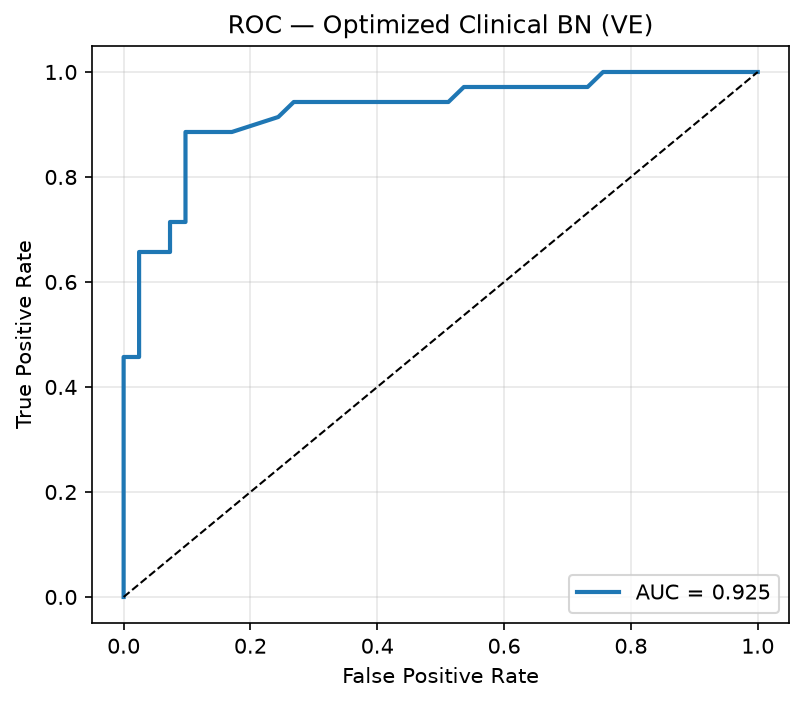
\includegraphics[width=\linewidth,height=0.74\textheight,keepaspectratio]{figures/fig4_roc_best.png}\\[0.2em]
    {\small\textbf{ROC Curve --- Optimized Clinical BN}}
    \column{0.46\textwidth}
    \centering
    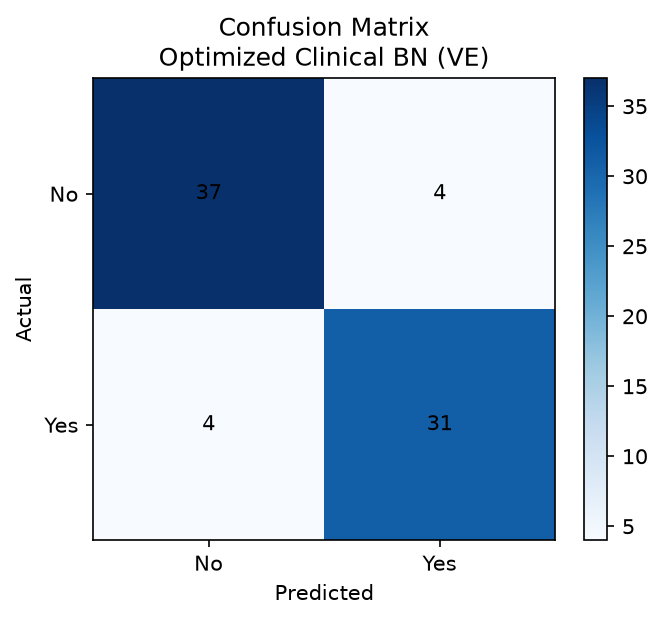
\includegraphics[width=\linewidth,height=0.74\textheight,keepaspectratio]{figures/fig3_confusion_best.png}\\[0.2em]
    {\small\textbf{Confusion Matrix --- Test Set}}
  \end{columns}
\end{frame}

% --- 16. Streamlit -----------------------------------------------------------
\begin{frame}{Interactive Streamlit Demo}
  \begin{columns}[T]
    \column{0.55\textwidth}
    \textbf{Six tabs} for live instructor demo:
    \begin{enumerate}
      \item \textbf{Diagnosis} --- $P(\text{Heart Disease}\mid\text{evidence})$, threshold slider
      \item \textbf{Metrics} --- accuracy, precision, recall, F1, ROC-AUC
      \item \textbf{Analysis Gallery} --- EDA, CPT, inference figures
      \item \textbf{Algorithm Lab} --- VE vs Belief Propagation
      \item \textbf{Network Explorer} --- DAG + metrics table
      \item \textbf{PGM Guide} --- three-pillar walkthrough
    \end{enumerate}
    \vspace{0.4em}
    \begin{block}{Recommended demo flow}
      Preset \textbf{Classic angina (high risk)} $\rightarrow$ \textbf{Compare all 4 models} $\rightarrow$ different $P(\text{Yes})$ per BN
    \end{block}
    \begin{block}{Deploy}
      \small
      Live demo: \url{https://heartdiseasepredictiondemo.streamlit.app/}\\
      Repo \texttt{Heart\_disease\_prediction\_in\_Probablistic\_graphical\_model}, main file \texttt{streamlit\_app.py}
    \end{block}
    \column{0.43\textwidth}
    \begin{tcolorbox}[title=Features]
      \begin{itemize}
        \item Human-readable clinical inputs
        \item \textbf{Directed DAG} (parent $\rightarrow$ child)
        \item Compare all 4 BNs side-by-side
        \item VE vs BP + sensitivity analysis
      \end{itemize}
    \end{tcolorbox}
  \end{columns}
\end{frame}

% --- 17. Discussion & Conclusion ---------------------------------------------
\begin{frame}{Discussion, Limitations \& Conclusion}
  \begin{columns}[T]
    \column{0.48\textwidth}
    \begin{block}{Findings}
      \small
      \begin{itemize}
        \item Manual Structure BNs excel at \textbf{interpretability}
        \item Data-driven trees improve \textbf{accuracy}
        \item Cleveland-focused model reaches $\geq$85\% on all metrics
        \item Exact BN inference is fast ($\sim$1\,ms)
      \end{itemize}
    \end{block}
    \begin{alertblock}{Limitations}
      \small Educational only; discretisation loss; Naive Bayes independence assumption.
    \end{alertblock}
    \column{0.48\textwidth}
    \begin{block}{Conclusion}
      \begin{itemize}
        \item Complete PGM system: Representation, Learning, Inference
        \item Four BN models + deployable Streamlit demo
        \item Optimized Clinical BN: \textbf{89--93\%} across all metrics
        \item Open source on GitHub
      \end{itemize}
    \end{block}
  \end{columns}
\end{frame}

% --- 18. Thank you -----------------------------------------------------------
\begin{frame}[plain]
  \begin{center}
    \vspace{1cm}
    {\Huge\bfseries\color{AAUBlue} Thank You}\\[0.5cm]
    {\Large Questions \& Discussion}\\[1cm]
    {\large Abiy Alemu \quad\textbar\quad Natnael Abayneh}\\[0.25cm]
    {\normalsize Addis Ababa University --- M.Sc.\ in Artificial Intelligence}\\[0.9cm]
    \begin{tcolorbox}[width=0.78\textwidth, colframe=AccentTeal, title=Resources]
      \small
      GitHub: \url{https://github.com/Natiabay/Heart_disease_prediction_in_Probablistic_graphical_model}\\
      Streamlit: \url{https://heartdiseasepredictiondemo.streamlit.app/} \quad|\quad Dataset: UCI Heart Disease \quad|\quad Tools: Python, pgmpy, Streamlit
    \end{tcolorbox}
  \end{center}
\end{frame}

\end{document}
